%!TEX root = ../../Heun_Dale_Haney_A_dynamic_approach_to_input_output_modeling.tex
%%%%%%%%%%%%%%%%%%%%% chapter.tex %%%%%%%%%%%%%%%%%%%%%%%%%%%%%%%%%
%
% sample chapter
%
% Use this file as a template for your own input.
%
%%%%%%%%%%%%%%%%%%%%%%%% Springer-Verlag %%%%%%%%%%%%%%%%%%%%%%%%%%
%\motto{Use the template \emph{chapter.tex} to style the various elements of your chapter content.}
\motto{In a complex and wealthy country like the United States, 
providing information on the structure of the economy and the environment 
is an essential function of government. 
It deserves more support.~\emph{\cite[p.~49]{Nordhaus:1999aa}}

\hfill---\emph{William D. Nordhaus}}

%%%%%%%%%%%%%%%%%%%%%%%%%%%%%%%%%%%%%%%%%%%%%%%%%%%%%%%
%%%%%%%%%% Conceptual and Theoretical Isseus %%%%%%%%%%
%%%%%%%%%%%%%%%%%%%%%%%%%%%%%%%%%%%%%%%%%%%%%%%%%%%%%%%
\chapter{Unfinished Business: Practical, Methodological, and Theoretical Issues}
% Always give a unique label
\label{chap:unfinished_business}
% use \chaptermark{} to alter or adjust the chapter heading in the running head
\chaptermark{Issues}
%%%%%%%%%%%%%%%%%%%%%%%%%%%%%%%%%%
%%%%%%%%%%%%%%%%%%%%%%%%%%%%%%%%%%
%%%%%%%%%%%%%%%%%%%%%%%%%%%%%%%%%%

%% \abstract{Each chapter should be preceded by an abstract (10--15 lines long) that summarizes the content. The abstract will appear \textit{online} at \url{www.SpringerLink.com} and be available with unrestricted access. This allows unregistered users to read the abstract as a teaser for the complete chapter. As a general rule the abstracts will not appear in the printed version of your book unless it is the style of your particular book or that of the series to which your book belongs.\newline\indent
%% Please use the 'starred' version of the new Springer \texttt{abstract} command for typesetting the text of the online abstracts (cf. source file of this chapter template \texttt{abstract}) and include them with the source files of your manuscript. Use the plain \texttt{abstract} command if the abstract is also to appear in the printed version of the book.}

%% Use the template \emph{chapter.tex} together with the Springer document class SVMono (monograph-type books) or SVMult (edited books) to style the various elements of your chapter content in the Springer layout.

\abstract*{This chapter reviews our list of unfinished business.
We begin by reviewing our call for better data collection and reporting
and expanding the discussion of metaphors and models. 
Thereafter, we call for new approaches
to ascribe value to material flows between the economy and the biosphere.
The remainder of this chapter discusses several questions
and methodological issues, including
hybridized EI-O and process methods,
resource quality, and co-products.
Then, several questions were posed:
are people capital stock?
what about the Sun? and
what is endogenous?
In all of the these areas, we called for additional 
inquiry and research 
into the questions raised by our framework.}


With any endeavor of this magnitude, 
namely development and presentation 
of a comprehensive framework for economies of the world,
unfinished business is inevitable. 
This chapter discusses several 
practical, methodological, and theoretical issues
that should be addressed in the future.
On a practical level, additional data are needed 
to fully utilize the framework developed herein.
In terms of methodological issues, the issue of co-products 
needs to be addressed.  
Finally, several theoretical issues, including
theories of value,
material and energy quality, 
boundaries, and 
the Sun
are addressed.
We begin with the issue of data.


%We begin with metaphors and models.


% %%%%%%%%%% Metaphors and models %%%%%%%%%%
% \section{Metaphors and models}
% \label{sec:metaphors_and_models}
% %%%%%%%%%%
% 
% This section circles back to the discussion that began the book and re-examines
% the importance of metaphor in light of the implications in the previous chapter.
% Historically, mainstream economists have used the \emph{machine} metaphor
% to describe economies. 
% In fact, much of mathematical economic modeling today 
% relies upon mechanistic conceptual foundations whose roots 
% are in Newtonian physics
% and The Enlightenment.\footnote{The subfield 
% 	of longwave economic growth modeling, as an example, 
% 	uses mechanistic language to describe their equations. 
% 	Jones~\cite[pp.~6 \&~18]{Jones:2001wn} 
% 	refers to the ordinary differential equations 
% 	that describe births, deaths, and the production of ideas
% 	as ``laws of motion.''}
% If your metaphor is a machine, it makes sense to analyze economies
% with equations that describe machines.
% In the mainstream, such equations usually, but not exclusively or restrictively,
% are developed assuming that the economic machine is a \emph{isolated} system.
% 
% In this book, we take the strong position that economies are
% better-represented as open, organic organisms with active metabolisms.
% Many ecological economists, 
% who are predisposed to view the economy as metabolic,
% reject the use of mechanistic equations 
% to describe the economy, in part because such equations often assume a 
% machine that operates independently from the biosphere.
% Other ecological economists dismiss mainstream economics 
% and its mechanistic models out of hand. 
% For example, S{\"o}llner pejoratively says 
% ``The prime example of physics envy and the desire 
% to emulate the natural sciences is, of course, 
% neoclassical economics which was explicitly and purposefully 
% copied from classical mechanics.''~\cite[p. 178]{Sollner:1997wx}
% 
% But, it doesn't have to be this way.
% We claim that it is not the use of equations 
% and mathematical models themselves that is the problem.
% Rather, it is the application of such equations 
% to an assumed isolated system
% that is is worthy of criticism.
% Thus, our approach herein includes rigorous application of the 
% admittedly mechanistic accounting equations 
% for materials, energy, embodied energy, and economic value
% \emph{under the assumption of} and \emph{including} 
% vigorous and necessary interactions between
% the economy and the biosphere.
% 
% It is our hope that this book allows
% 
% \begin{itemize}
% 	\item{mainstream economists to see that}
% 	\begin{itemize}
% 		\item{the metabolism metaphor is apt because 
% 		interaction between the economy and the biosphere is 
% 		what drives economic growth and}
% 		\item{rigorous mechanistic models can and should include 
% 		interactions between the biosphere and the economy; and} 
% 	\end{itemize}
% 	\item{ecological economists to see that rigorous mathematical modeling
% 	is an important tool for understanding interactions
% 	between the economy and the biosphere.}
% \end{itemize}
% 
% We encourage both mainstream and ecological economists
% to embrace mathematical modeling of 
% material, 
% energy, 
% embodied energy, 
% and economic value flows
% both within the economy and between the economy and the biosphere
% as a valid method of inquiry for modern economics.
% And, we encourage continual assessment of our models and metaphors.
% The stories we tell ourselves about our world have a significant 
% impact on how we perceive the world.
% We had better get those right.


%%%%%%%%%% Data %%%%%%%%%%
\section{Data}
\label{sec:Data}
%%%%%%%%%%

In Chapter~\ref{chap:intro}, 
we noted the importance of ``counting''
materials, energy, and value as each flows through economies.  
Unfortunately, unless data on these flows 
is collected and disseminated routinely, 
such counting is impossible.
At several points in this manuscript,
we have noted the very practical issue of the
need for additional data, information, and analysis.

In Section~\ref{sec:materials_auto},
our attempt to account the physical flows of 
materials through the US auto industry was
severely hampered by the lack of any data on
material flows.
Work to account such flows is starting to be
addressed at the level of economies,
particularly within Europe.\cite{EUROSTAT2011}
This work needs to continue, but
sub-economy, inter-industry material accounts need to be developed, too.
Chapter~\ref{chap:intensity} noted the need to collect
data on human and draught animal physical work input to 
sectors of economies, espeically for those economies where 
muscle work is on the same order of magnitude 
as fossil fuel energy input.

The need for rigorous and accurate data
is all the more pressing in light of the need 
to track physical capital in sectors,
as suggested in Chapter~\ref{chap:intensity}.
If this accounting relies on process-type
analysis,
then there is a critical need for systematic
collection and public dissemination of such data.
Some of these data are available only in proprietary format;
e.g., the latest version of the ecoinvent database (v3)
contains detailed analysis of over 10,000 
processes.\cite{EcoInvent2012}
This is a fantastic effort, but more needs to be
done to bring this crucial information into the public arena.

Environmental economic accounting in the US national accounts is currently non-existent. 
It was suspended by congress after the first
tables were published and has been on hold for twenty years. 
The BEA developed the
Integrated Environmental and Economic Satellite Accounts 
to complement the national accounts and track the 
``interactions of the economy and the environment.''~\cite[p.~33]{BEA1994a} 
In 1994, the BEA published the first phase of tables, for subsoil resources, 
along with detailed economic accounting 
and environmental valuation methodology behind the new data.\cite{BEA1994a, BEA1994b} 
The first set of tables valued the stock of
subsoil assets: oil, gas, coal, metals, 
and some major nonfuel minerals for the years 1947 to 1991. Each
year of data included values for \emph{Opening stock}, 
\emph{Additons}, \emph{Depletion}, \emph{Revaluation adjustment}, 
and \emph{Closing stock}. 
Several alternative valuation methods were used to provide a range of estimates.

Unfortunately, Congress ordered the BEA
to suspend all work
on environmental accounting, including development of
additional accounts for renewable and environmental resources.  
Congress asked for an independent panel of scientists to review the 
BEA's methodology.
In 1999, the review panel submitted its thorough evaluation as well as its strong
recommendation that the BEA
be funded to continue its work.\cite{Nordhaus1999a}
William Nordhaus,
chair of the panel, summarized the panel's recommendations 
in the lead quote for this chapter, 
``In a complex and wealthy country like the United States, 
providing information on the structure of the economy and the environment 
is an essential function of government. 
It deserves more support.''~\cite[p.~49]{Nordhaus:1999aa}
Fifteen years later, Congress has yet to act on this recommendation 
and lift the embargo on environmental accounting.

The business axiom ``you can't control what you don't measure''
seems appropriate here. 
As the world confronts significant challenges
of material and energy supplies in the coming years,
it will be impossible to make wise decisions about
which materials to use,
which energy sources to develop, and 
which products to incentivize.

The lede quote for Chapter~\ref{chap:value}
(``We try to measure what we value. 
We come to value what we measure.''~\cite[p.~2]{Meadows:1998aa})
points out that we are not presently valuing highly enough
the important flows that describe our metabolic economies.
We add our voices to those encouraging governments and 
institutions to collect high-quality data on material 
and energy flows.


%%%%%%%%%% Theories of value %%%%%%%%%%
\section{Theories of value}
\label{sec:theory_of_value}
%%%%%%%%%%

As stated in Chapter~\ref{chap:value}, mainstream economics assumes a
\emph{subjective} theory of value, 
in which value is determined by the relative ability 
of products to satisfy the wants of buyers and sellers alike.
However, a person's wants are malleable and are, in turn, formed within a 
``constellation of shared goals to which a society aspires.''~\cite{Costanza:2004we}
Thoughout history, economists (particularly the classicals) 
and non-economists have searched for an invariant, objective, 
\emph{intrinsic} determinant of value.\footnote{Following the ecological economics literature, 
	we use the term intrinsic in the sense of ``objective.'' Costanza~\cite{Costanza:2004we} 
	notes that a better term would be objective in order to avoid moral overtones associated 
	with the term intrinsic.} 
Adam Smith, Karl Marx, David Ricardo, and neo-Ricardian Piero Sraffa all proposed 
alternative determinants of value.  
Their proposed objective theories of value were based 
on identifying the primary input into production,
such as \emph{labor} (Marx) or \emph{land} (Malthus), 
and using that input in the sense of a numeraire, 
a way to measure value across the entire spectrum 
of goods and services in commensurate units.

Costanza~\cite{Costanza:2004we} makes the case for energy 
as the only truly primary input into production 
and thus an, or rather \emph{the}, objective determinant of value. 
On a global scale, he notes, (solar) energy 
(including that which is stored in fossil fuels) is 
the only primary input into production:
everything else is an intermediate input. 
Thus, free energy input to production (accounting for all upstream energy)
could be the basis for an objective (intrinsic), 
energy theory of value.\footnote{This line 
	of inquiry has yielded some interesting analysis of the amount 
	of solar energy required to run the economy. 
	See Section~\ref{sec:emergy} for further discussion of the concept of \emph{emergy}.}
However, mainstream economics has rejected an energy theory of value, 
in favor of the subjective theory of value discussed in Section~\ref{sec:Value_Methodology}.
Because energy intensity ($\boldsymbol{\varepsilon}$) 
and the Energy Input-Output (EI-O) method 
were significant aspects of the 
proposal for an energy theory of value, 
many mainstream economists spurn 
analyses aimed at determining~$\boldsymbol{\varepsilon}$.

In contrast, we observe that energy intensity 
does not necessarily lead to an energy theory of value
and claim that energy intensity is inherently useful
as a metric describing the energy pathways traveled by economic products.
Energy intensity can provide important information for purchasing decisions
in increasingly interconnected economies.

In the development of our framework, we used the subjective theory of value 
(i.e., value based on market prices at the time of transaction) 
for pragmatic, rather than philosophical, reasons.
We believe that the information and signals provided by markets and prices 
are not sufficient to guide economies situated within a ``full'' earth.
And, national economic accounting limits its focus to measuring value-added, 
but ignores that to which value is being added,
thereby distorting economic value flows. 
As easily accessible forms of energy (e.g.,  oil extracted from the Texas panhandle) 
are used up and more difficult locations must be tapped (e.g., Alaskan north slope) 
the economy appears to grow.
The ``value-added'' by human and manufactured capital increases, 
as humans must do more work to extract domestic energy sources. 
However, what is actually happening is that the stock 
of natural resource is diminishing, 
and the drawdown of natural capital is mis-measured by GDP as income.\cite[pp.~66~and~75]{Daly1997}

Therefore, as ``that to which value is added'' diminishes, 
economic growth begins to reach binding constraints. 
Identifying the optimal economic 
scale---rate of materials put through the economy---that 
is viable for the biosphere to handle becomes an optimization problem. 
However, this is an optimization 
problem that the market is unable to solve on its own. 

Our framework provides a natural starting place for extending 
existing economic analysis methods to better
guide economies situated within a ``full'' earth. 
Instead of turning to an energy theory of value,
a system of envrionmental-economic accounting 
could be put in place to estimate the value 
of flows to and from the biosphere.\footnote{As of this printing, 
	the System of Environmental-Economic Accounting (SEEA)~\cite{UNSEEA:aa}
	is in its third revision 
	using a process of global consultation. 
	This system contains internationally agreed-upon standards for quantifying value flows 
	to and from the biosphere. 
	SEEA is a system analogous to the System of National Accounts (SNA), 
	a framework for measuring economic value creation consistently across nations.} 
Such a system could be included in our framework
to reconnect the economy to the biosphere, 
and flows that were conspicuously 
absent from Figure~\ref{fig:basic_value} will
be included, as shown in Figure~\ref{fig:basic_value_with_biosphere_flows}.

\begin{figure}[ht!]
\centering\
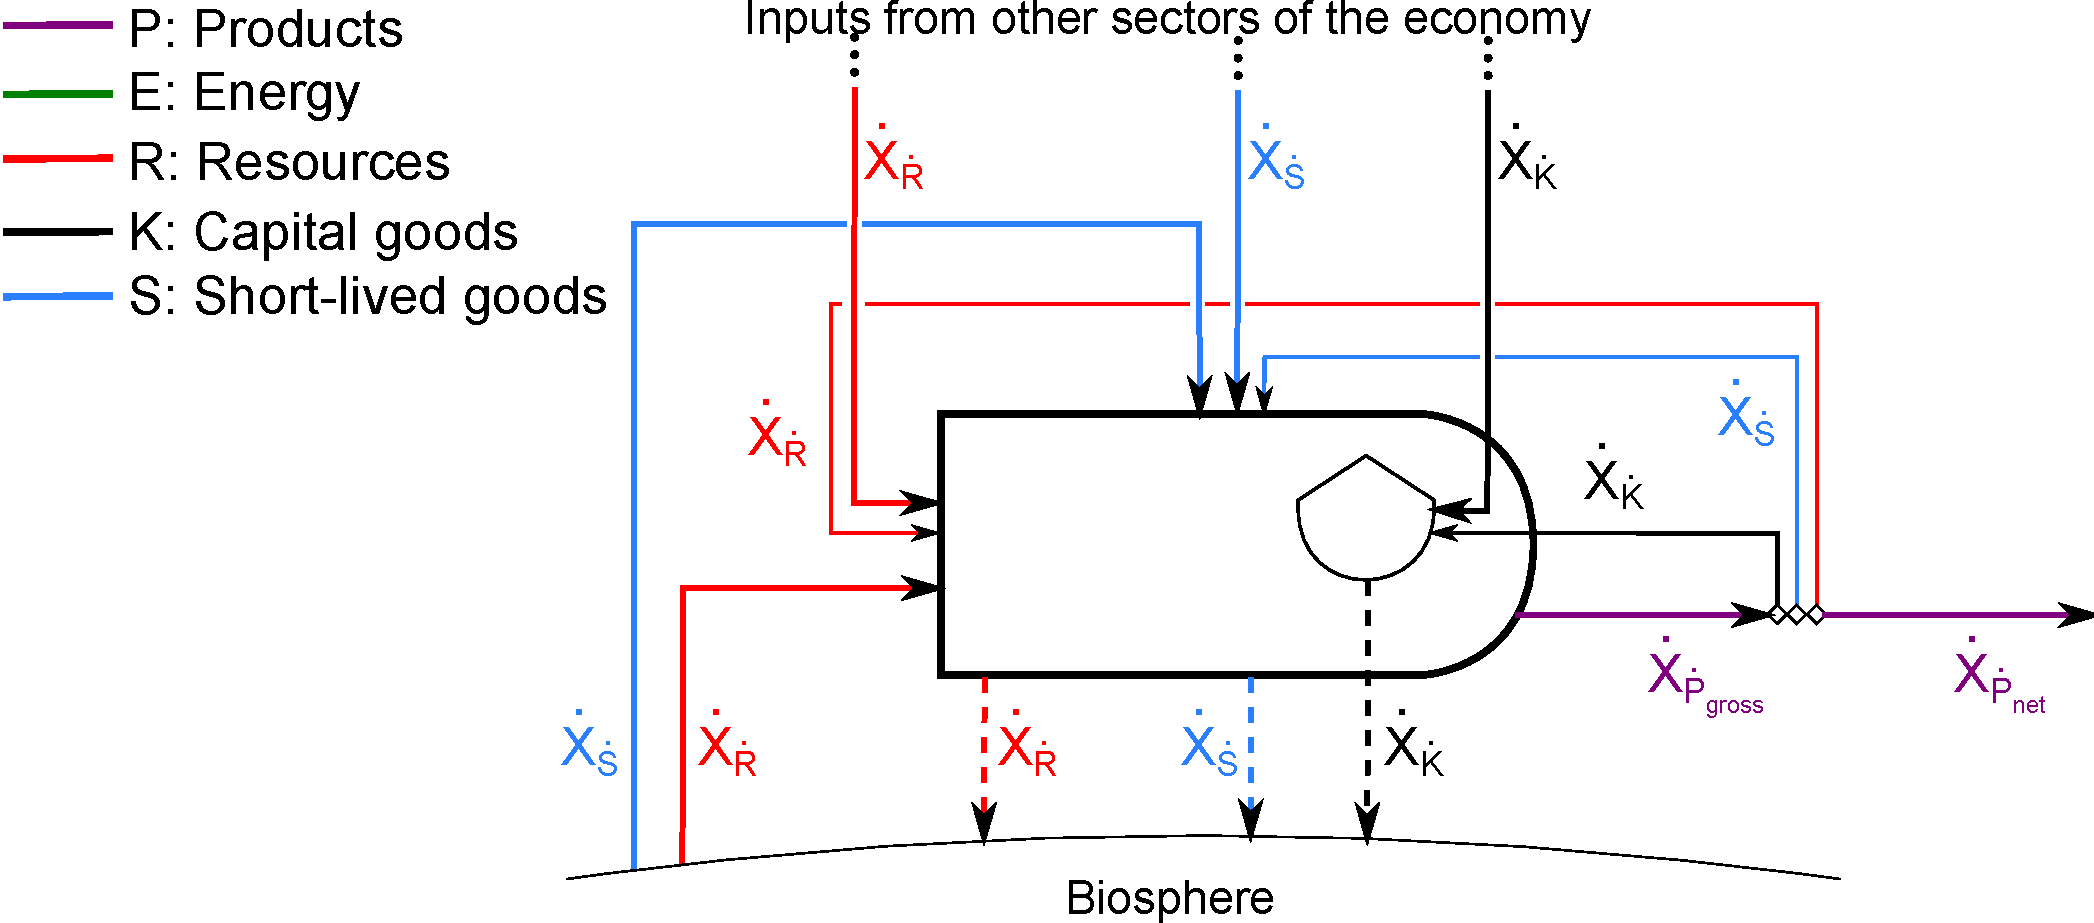
\includegraphics[width=0.8\linewidth]{Part_3/Chapter_Unfinished/images/PERKS_basic_unit_value_with_biosphere_flows.pdf}
\caption[Aggregated flows of value for a single sector including flows to and from the biosphere]{Aggregated flows of value for a single sector including flows to and from the biosphere.}
\label{fig:basic_value_with_biosphere_flows}
\end{figure}


%%%%%%%%%% Hybrid %%%%%%%%%%
\section{Hybrids of I-O and process-based methods}
\label{sec:hybrid}
%%%%%%%%%%

In early chapters,
we made the distinction between
process-based (often called ``bottom-up'') 
and Input-Output (often called ``top-down'')
analyses.
The advantages and disadvantages of each type
of analysis are outlined in Figure~\ref{fig:IO_vs_process}.

Process analysis is based on detailed technological
or engineering models of specific economic processes.
Model specification and data collection is arduous,
time-consuming,
and costly.
The aim of process analysis is to calculate the
energetic and material flows associated with the process
under study by disaggregating the process into
several components or sub-processes.
In reality,
any economic process exists as part of a complex network of
interacting processes that encompass the entire economy.
Bullard et al.\ said 
``each step in a process analysis may be viewed as 
an expansion of the system boundary 
(around the item being analyzed) 
into the economic system.''~\cite[p.~281]{Bullard:1978vd}
Figure~\ref{fig:Hybrid_boundary} shows that 
every process calls on every other process within the economy,
even if only minutely and indirectly at many steps removed.
Obviously,
the time, 
effort,
and cost involved with trying to model and
measure all of the flows involved becomes daunting
for even low numbers of interacting processes.
The decision of where to draw the boundary of
a process analysis is known in the 
lifecycle assessment literature as the 
\emph{truncation problem}.\cite{Suh2004}
One method to extend the comprehensiveness of process
analyses is to use a hybrid method,
utilizing data from an EI-O analysis to supplement the
missing data from the truncation of the process analysis.
The financial cost of goods and services identified by
the process analysis are converted to energy
(or material) flows via the EI-O method.
The truncation error is replaced by a smaller aggregation
error due to limitations of the EI-O 
method.\cite{Bullard:1978vd}
A variety of other hybrid methods exist which also aim to
overcome the limitations of either process or I-O method 
individually.\cite{Bullard:1978vd, Suh2004, Suh2002, 
Crawford2008, Zhai2010}

\begin{figure}[p]
\centering\
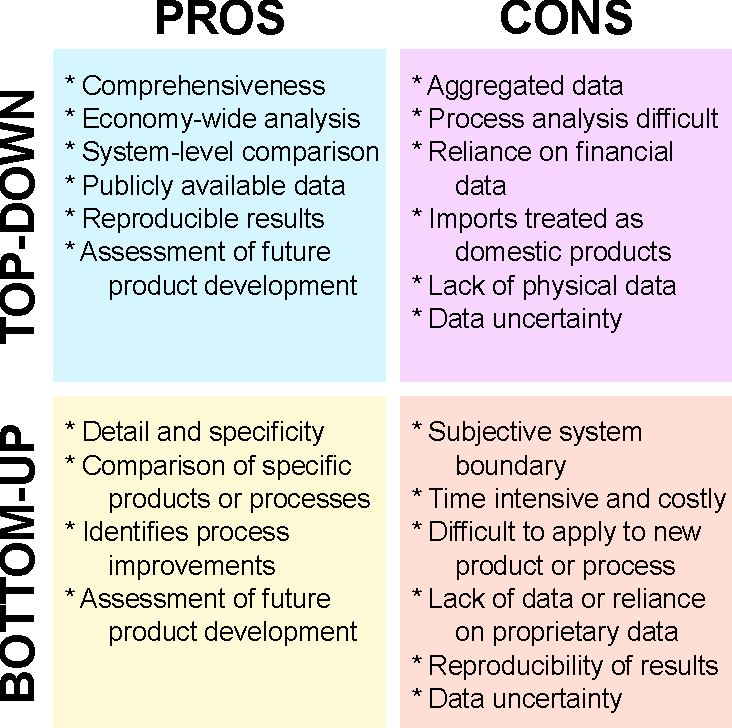
\includegraphics[width=0.8\linewidth]{Part_3/Chapter_Unfinished/images/Top_down_vs_bottom_up.pdf}
\caption[Top-down vs.\ bottom-up analyses]{Advantages (pros) and disadvantages (cons) of ``top-down,'' I-O and ``bottom-up,'' process-based analyses, adapted from~\cite{Hendrickson2006}.} % chktex 38
\label{fig:IO_vs_process}
\end{figure}

\begin{figure}[p]
\centering\
\includegraphics[width=\linewidth]{Part_3/Chapter_Unfinished/images/Hybrid_boundary.pdf}
\caption[System boundary for process and I-O analyses]{System boundary for process and I-O analyses, adapted from~\cite{Bullard:1978vd}.}
\label{fig:Hybrid_boundary}
\end{figure}

At several points in this book,
we noted the need to track accumulation of embodied
energy in sectors of the economy.
It may be that process-based methods are best for doing so.
However, we realize the limitations of process-based
methods (time, cost, etc.).
Perhaps hybrid methods can provide the necessary 
data without the high 
cost of a full process-based approach.


%%%%%%%%%% Second Law %%%%%%%%%%
\section{Resource quality and irreversibility}
\label{sec:resource_quality_and_irreversibility}
%%%%%%%%%%

The quality of both materials
and energy play a role in the 
efficiency with which economies 
convert material resources into products.

Raw material and energy resources must first 
be extracted from the natural environment 
before they are utilized in the economy 
to provide goods and service to society. 
Despite increasing levels of technological efficiency, 
for example in consumer goods such as refrigerators and cars, 
evidence shows that 
the energy intensity of primary resource extraction, 
i.e.\ the energy required to extract raw materials 
from the environment, 
has been steadily increasing over 
the last fifty years.\cite{Hall1986, Mudd2010, Brandt2011} 
This increasing energy requirement for 
primary extraction means that 
less \textit{net energy} is available 
for downstream uses. 
%**** Mik---Add a discussion here that links 
%EROI (Chapter 3, Example B) with resource quality. ****
An important metric in this regard is
\emph{energy return on investment}~(EROI),
outlined in Section~\ref{sec:B_energy},
which measures the energy production
\emph{per unit} of energy investment by society.
As resource quality declines,
more energy is needed to extract resources,
EROI decreases,
and there is less net energy available to society.
If this decline in net energy availability 
outpaces technological advances in energy efficiency, 
there may be deleterious impacts on the 
economic output of the economy.

Within our framework, we do not account for either
the material or energetic quality of resources 
that pass through the economy nor the 
irreversibility of economic processes.
The following two subsections (\ref{sec:energy_quality}
and~\ref{sec:material_quality}) briefly discuss energy and material quality.
Thereafter, we raise the issue of thermodynamic irreversibility.



%+++++++++ Energy Quality ++++++++++
\subsection{Quality of energy}
\label{sec:energy_quality}
%+++++++++

The First Law of Thermodynamics
tells us that
the quantity of energy is conserved in every process.
The First Law
does not speak about the quality of energy---not
all forms of energy are equally \emph{useful}.
For instance,
a bath-full of water has as much thermal energy
as can be provided by a pint~(half liter) of
gasoline.\footnote{This assumes a 230 liter bath at
40$^\circ$ C,
i.e.\ 20$^\circ$ C above ambient.}
However, the gasoline is a much higher quality
store of energy than the water.
It is much more useful for performing tasks.

There are several ways to assess the quality of energy.
The Second Law of Thermodynamics provides, 
among other things,
a framework for discussing the \emph{quality} of energy.
Hammond and Winnett~\cite{Hammond:2009tu} reviewed
the influence of thermodynamics on ecological economics 
and noted the importance of the concept of \emph{exergy},
which combines the First
and Second
Laws of thermodynamics
to describe the maximum physical work 
which can be performed by an energy resource
in coming into equilibrium with its environment,
stating that exergy:

\begin{quote}
	represents the thermodynamic `quality' 
	of an energy carrier, 
	and that of the waste heat or energy lost in the reject stream. 
	Electricity, for instance, 
	may be regarded as an energy carrier having a high quality, 
	or exergy, because it can undertake work. 
	In contrast, low temperature hot water, 
	although also an energy [re]source, 
	can only be used for heating purposes. 
	This distinction between energy~(strictly enthalpy) 
	and exergy is very important 
	when considering a switch, for example, 
	from traditional internal combustion engines 
	to electric, hybrid, or fuel cell vehicles. 
	Thus, \ldots{} it is important to employ exergy analysis 
	alongside a traditional First Law energy analysis 
	in order to illuminate these issues.
\end{quote}

As such, exergy is a measure of how far a resource
is from thermodynamic equilibrium with its environment.
The further a resource is from equilibrium with the 
environment---the biosphere---the
higher the exergy and the higher the quality of the resource.

The quality of energy can be assessed in terms of economic value, too.
Some energy resources, such as liquid fuels, 
are more economically valuable than others,
i.e.\ within society, there is a preference for these resources,
such that, ``accounting for energy quality reveals a relatively strong relationship 
between energy use and economic output.''~\cite[p. 313]{Cleveland2000}
We see this preference played out on a daily basis
when coal is converted to electricity at 
an average efficiency of around one third.
Society is willing to pay a premium for electricity
over coal due to its vastly superior usefulness 
for a multitude of tasks.

%+++++++++ Material Quality ++++++++++
\subsection{Quality of materials}
\label{sec:material_quality}
%+++++++++

% **** Mik: Please review and add to this draft section. --Matt ****

%The concept of material quality has connections to our framework in two ways:
%\begin{enumerate}
%	\item 
%		first is Georgescu-Roegen's so-called 
%		``Fourth Law of Thermodynamics'';
%	\item		
%		second is (decline of) the quality of 
%		natural resources	within the biosphere.
%\end{enumerate}
%
%Georgescu-Roegen proposed a 
%Fourth Law of Thermodynamics
%\index{Fourth Law of Thermodynamics}
%which states that, ``In a closed system, 
%the material entropy must ultimately reach a maximum:'' 
%economic processes degrade material through wear and tear,
%just as energy.\cite{GeorgescuRoegen:1977tf}
%For example, consumption of coal to produce electricity
%results in CO$_2$ and ash that cannot
%be reprocessed into coal.
%Although mass (measured in kilograms) 
%is conserved through processes, 
%CO$_2$ and ash are significantly less useful than coal,
%and Georgescu-Roegen's ``Fourth Law'' 
%states that we need a way to account
%for the loss of material quality.
%
%The Fourth Law also states that,
%materials may never be recycled with 100\%
%efficiency, 
%hence to maintain a constant stock of material,
%some new resources must be imported into the system.
%In the case of the biosphere,
%materials are lost from the biosphere through
%the actions of tectonics and new materials are added
%via volcanic activity and erosion of rock by
%water, plants and animals.

Similar to energy resources, 
non-energy resources 
have a range of quality, despite being conserved
in mass through every process.
An intact brick is of higher material quality---is of more use---than
after it has been ground to dust and scattered on the wind.
Society relies on material stocks or flows 
that have been concentrated by natural biophysical processes,
for example mineral seams or water courses. 
We do not mine desirable material from locations with
the average abundance of crustal materials.
As with energy,
we may measure the material quality of a resource
in reference to its environment,
in this case,
the average chemical composition of
its environment.
The more concentrated the resource,
the further it is from chemical equilibrium
with the environment and the higher the quality.
Again, exergy is a measure of this kind of quality.
The further a resource is from chemical equilibrium
with its environment,
the higher the exergetic content.

Additionally,
it takes more energy to process less concentrated resources
and more total material must flow through 
the process~(including overburden---the wasted portion that is extracted)
and the greater wear and tear on equipment.
This additional processing requirement entails that 
we will likely never mine average crustal abundance for needed
materials, or mine gold from seawater.
Furthermore,
it also entails that recycling---the act
of turning low quality materials into
high quality resources---requires energy
and degrades equipment.
The lower quality the waste,
the more energy and degradation occurs
such that
one hundred percent recycling of materials
is almost certainly practically (and possibly theoretically) 
impossible.
As such, 
we can deduce that the economy \emph{must always} be
a subsidiary of the biosphere, \emph{open} to
flows of materials both from (resources) and 
to (wastes) the biosphere.
This fact has direct implications for dematerialization
of our economies, 
which was discussed in reference
to our framework in Section~\ref{sec:recycling}.
There are fundamental limits to the amount
of material that must be directed to desired
end services.
For example, automobiles 
must have a minimum level of embodied materials.\footnote{Note
that this minimum is likely many times lower than the 
mass of current automobiles,
which are driven largely by preference.
The Rocky Mountain Institute has done some
work on the ultra-light, 
``hypercar'' concept.\cite{RMI1996}}
Despite the drive to dematerialization
and the apparent ``unhooking'' of the
material and energy intensity of GDP,
much of the dematerialization of ``developed'' 
nations has been by exporting manufacturing
to other countries.\cite{allwood2012sustainable}
The material footprint of OECD nations, 
when weighted by consumption, 
has increased significantly since 1990.\cite{Wiedmann2013}

%Furthermore, initial extraction of easy-to-reach ores 
%and fossil fuel resources (coal and oil)
%leads, over time, to a reduction in the quality 
%of material resources 
%(ore grades decrease over time).\cite{Mudd2010}
%As the quality of these resources degrades,
%greater amounts of energy must be expended
%(resulting in greater degradation of capital equipment)
%during their extraction.


%+++++++++ Irreversibility ++++++++++
\subsection{Process irreversibility}
\label{sec:irreversibility}
%+++++++++
Our framework implicitly assumes, 
since we make no use of the Second Law,
that all economic processes could be run in reverse;
that products could be unmade into resources
and that the energy and other short-lived material
inputs would be spontaneously upgraded back into their
original form.
This of course is not true.
Irreversibility is the concept that naturally-occurring processes 
are uni-directional in time.
For example, 
bouncing a rubber ball heats it up;
heating up a rubber ball does not cause it to
spontaneously jump off the table.
%the flow of electrical current through a resistor
%generates heat;
%however, pointing an operating hairdryer at an electrical resistor 
%does \emph{not} produce electricity.

Considering the production of electricity from coal,
we note that two important processes within a power plant are \emph{irreversible}:

\begin{itemize}
	\item{the combustion process that converts coal to CO$_{2}$ and ash 
	(with associated thermal energy release, $\dot{Q}$) and}
	
	\item{the heat transfer process wherein $\dot{Q}$ flows 
	from high temperature to low temperature (with associated 
	mechanical work production).\footnote{Note 
		that the process of generating
		electricity via mechanical work is (at least in theory) a
		\emph{reversible} process.
		The generator could be run as a motor by electricity to produce
		mechanical work.
		In theory,
		electrical work and mechanical work are fully exchangeable;
		in reality, efficiency losses mean this is not quite the case.}}
\end{itemize}

\noindent{}Thermal energy does not spontaneously flow from low temperature to high temperature.
Neither do ash and CO$_{2}$ spontaneously combine to form coal.

The concepts of resource quality and irreversibility are inextricably linked.
One statement of the Second Law
indicates that heat flow is irreversible: 
it flows only from hot to cold. 
Because lower-temperature heat is less useful, 
we say that the thermal energy has 
degraded when it has been used~(comes 
into equilibrium with the environment).
Again,
exergy is a measure of irreversibility of processes.
Exergy cannot be created, it can only be destroyed,
hence a process is \emph{irreversible}
if exergy is destroyed during the process.\footnote{The concept of
irreversibility is often discussed in terms of \emph{entropy},
which can only be created and cannot be destroyed.
A process that generates entropy is said to be irreversible
and all real processes generate entropy.}

%The proposed Fourth Law is similar: 
%materials are degraded through their use.
%Georgescu-Roegen's proposed Fourth Law establishes an analogy between
%(a) the Second Law of Thermodynamics,
%in which energy quality degrades with use and
%(b) the Fourth Law of Thermodynamics,
%in which material quality degrades with use.\footnote{The analogy 
%	between the First and Fourth Laws of Thermodynamics
%	are similar to the analogy between 
%		(a) the Law of Conservation of Mass, 
%		in which mass can be neither created nor destroyed and 
%		(b) the First Law of Thermodynamics, 
%		in which energy can be neither created nor destroyed.}

%These factors could be incorporated by
%the concept of exergy, which may be used to measure
%both material and energetic quality.

Energy resources, such as coal, are useful
since they are far from equilibrium with their environment,
energy may be released into the environment by
splitting the carbon-carbon bonds to form 
carbon-oxygen bonds with free oxygen 
within the atmosphere.
The exergy content of the coal is destroyed during
the equilibration process.\footnote{Strictly speaking,
the exergy content of the coal is only fully destroyed
when the CO$_2$ and ash have dispersed to their average
concentration within the environment since,
in theory,
this diffusion~(which happens spontaneously) 
could be used to perform work.}

Similarly, high grade mineral ores, such as bauxite, 
are useful since they are far from equilibrium with their
environment---the average abundance of materials
within the earth's crust.
The chemical exergy of materials may be upgraded
during processing---bauxite is refined into pure 
aluminum---but only at the expense of a greater
amount of exergy destruction elsewhere---the coal
burned to generate the electricity---i.e.\ the process is irreversible.

% Add a little vertical space to indicate a summary
\vspace{5 mm}

We recommend that future work be done to incorporate 
concepts of resource quality and irreversibility 
into our framework by accounting for flows and
destruction of exergy within economic processes.


%%%%%%%%%% Make-Use %%%%%%%%%%
\section{Co-products}
\label{sec:make-use}
%%%%%%%%%%

Our materials, energy, and value accounting framework 
has been developed under the assumption 
that each economic sector makes a single product ($\dot{P}$).
This assumption dates from the early days of the EI-O method.\cite{Bullard-III:1975aa}
In particular, the matrix mathematics of Chapter~\ref{chap:intensity}
relies heavily on this assumption. 
However, in later years, the EI-O method was extended 
in the literature to include
co-products for each economic sector.\cite{Costanza:1984tq,Casler1984} 
To do so, both \emph{make} and \emph{use} data are employed.\footnote{The
	\emph{make-use} method is sometimes also called the
	\emph{supply-use} method.
	}

We decided to leverage the older,
single-product formulation of the EI-O method
for the purposes of simplicity. 
The materials, energy, and value accounting framework
presented herein is more easily understood 
without the additional complexity of the make-use formulation 
of the EI-O method.
However, work remains to adapt the framework
developed herein to the make-use formulation of the EI-O method.

%%%%%%%%%% Recycling %%%%%%%%%%
\section{Extending the methodology to include recycling and waste treatment}
\label{sec:recycling_and_waste}
%%%%%%%%%%

In the accounting framework presented in Chapters~\ref{chap:materials}-\ref{chap:intensity},
we assumed that all waste flows~($\dot{W}_{j0}$) and depreciated capital flows~($\dot{K}_{j0}$)
from economic sector $j$ flowed straight to the biosphere.
In general, this is not the case within the economy.
The Waste Management and Remediation Services sector (NAICS 562) has the responsibility,
within the US economy,
of collecting and disposing of wastes.
Additionally, much material is recycled within the economy 
(rather than being disposed into the biosphere)
and many capital goods are sold for re-use prior to recycling of materials,
for example second-hand cars and office equipment.

We may represent these flows of resources ($\dot{R}_{j}$), 
short-lived goods ($\dot{S}_{j}$), and capital goods ($\dot{K}_{j}$)
as flows other than the product flow ($\dot{P}_{j}$)
leaving sector $j$
as in Figure~\ref{fig:PERKS_waste}.

\begin{figure}
	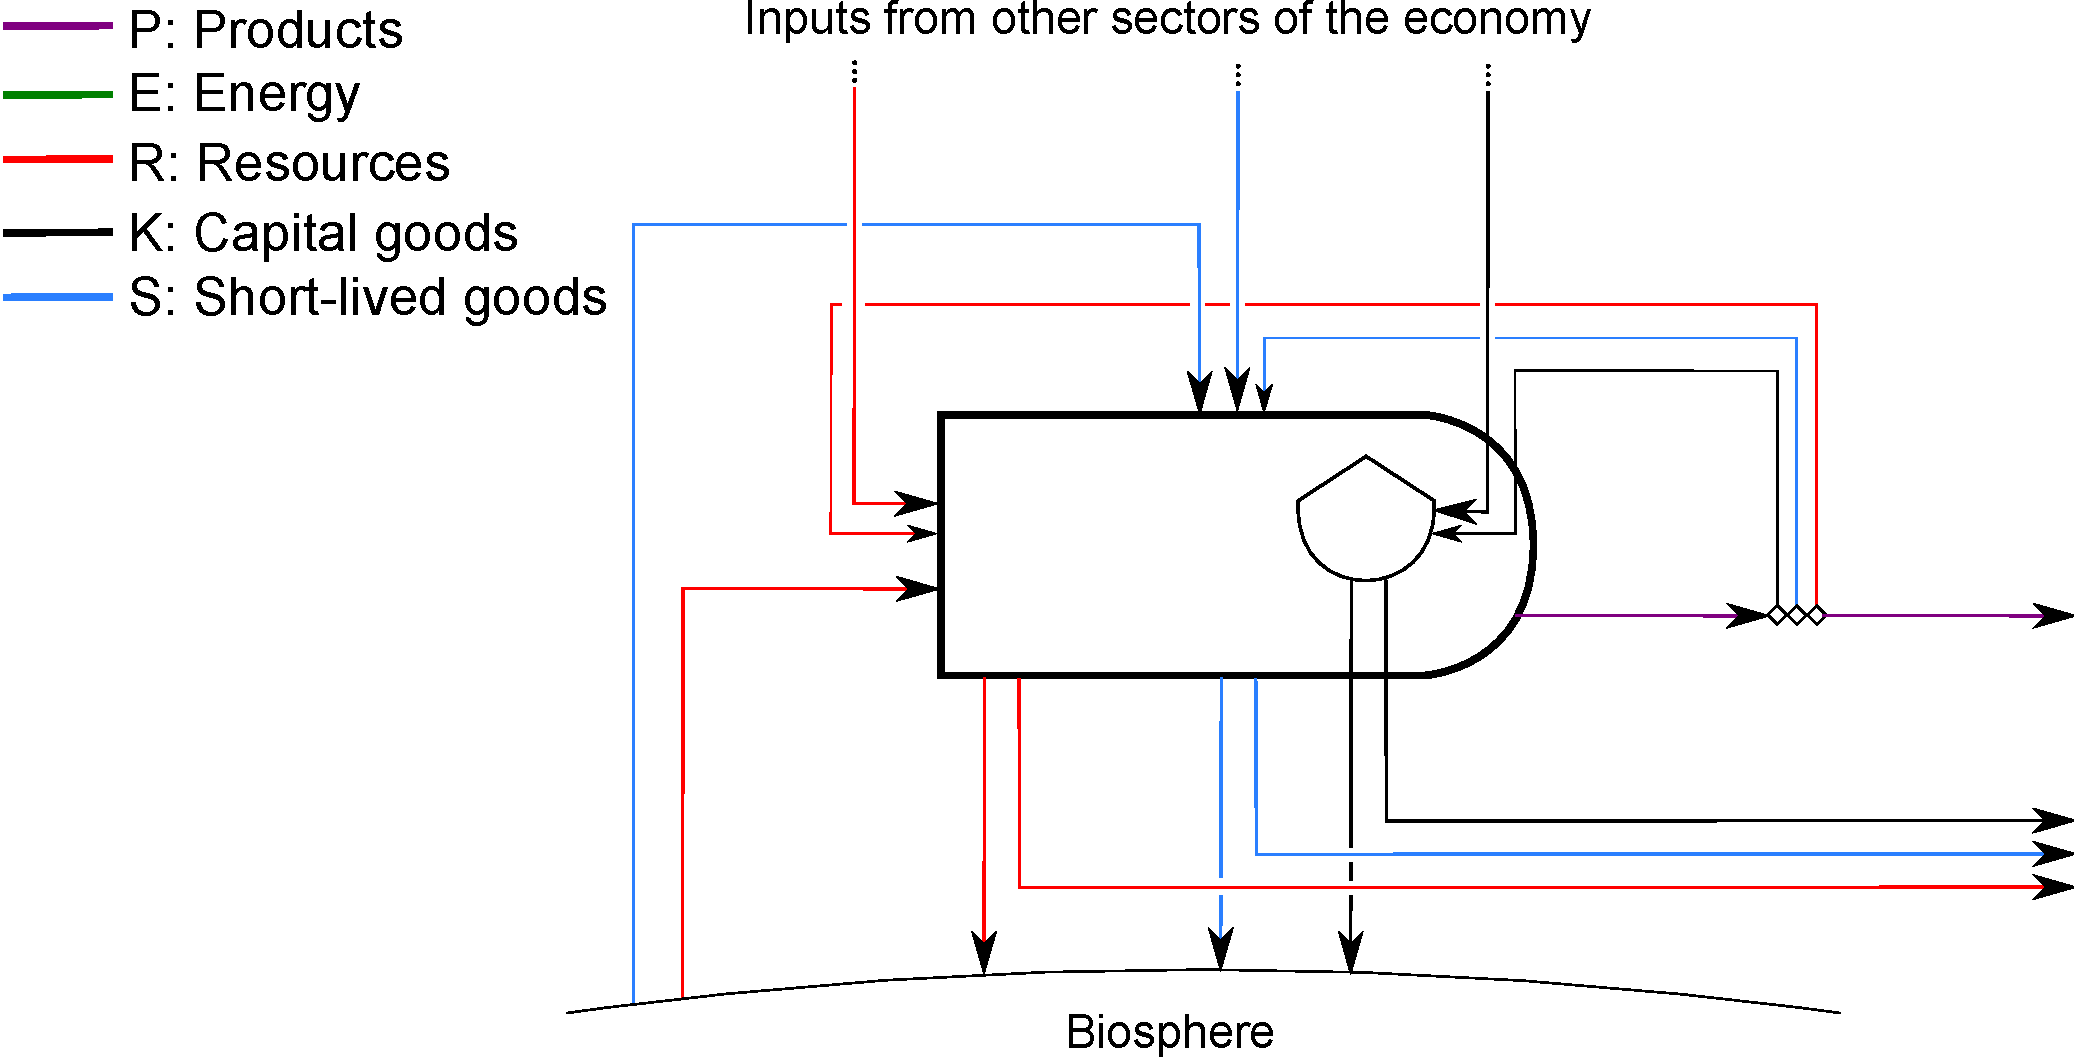
\includegraphics[width=\linewidth]{Part_3/Chapter_Unfinished/images/PERKS_basic_unit_materials_recycle.pdf}
	\caption[Material flows through an economic sector with waste treatment]{Material flows 
					through an economic sector with waste treatment flows to other economic sectors.}
	\label{fig:PERKS_waste}
\end{figure}

Such flows violate the `one sector-one product' assumption of the Leontief inversion method.
Methods based on make-use tables,
as developed by von Neumann~\cite{vonNeumann1945} and Sraffa~\cite{Sraffa1960}
are able to account for multiple products from each sector.

%%%%%%%%%% People as capital stock %%%%%%%%%%
\section{Are people capital stock?}
\label{sec:people_as_stock}
%%%%%%%%%%

%**** Mik: complete this section. ****
There is an open
question as to what sort of \emph{stuff} 
should be included within the capital
that accumulates in society. 
Should the material constituting literal
\emph{human capital}---human bodies---be included? 
If humans are to be included within $K_{1}$, 
some resource flow~($\dot{R}_{i1}$)
must be converted into 
human capital flow~($\dot{K}_{11}$)
which then adds to the stock of human capital~($K_{1}$)
within society.
This resource flow is food.
Food itself represents a large ``resource''
flow and has a large associated energy content. 
Additionally, 
within industrial economies, 
a large amount of energy resources 
are channeled toward the production of food, 
meaning that the \emph{embodied energy}
of food may actually be several times larger than
the direct energy content of the food itself. 

Further questions arise. 
What is the ``product'' of society? 
A materialistic view might hold that the product of
society is human bodies and the labor they can accomplish. 
If so, 
should the agriculture industry 
be accounted as part of the energy sector 
because its aim is to provide 
an energy service (labor)? 
For non-industrial, agrarian societies, 
the proportion of total energy flow 
comprised by manual (or draught) energy 
may be large. 
In industrialized societies, 
it may be negligible, 
however, 
the energy flows necessary to support agriculture
may be many times larger than the food energy
(and certainly many times larger 
than the labor energy) 
delivered, therefore entailing an EROI of less than unity. 
Agrarian societies are necessarily constrained 
by the fact that the energy content of the food delivered 
\emph{must be} greater than the labor (and draft) 
energy required to produce it.

Another view is that societal capital~($K_{1}$) 
includes only man-made capital, 
i.e.\ items manufactured by humans,
but not humans themselves. 
For the purposes of the framework outlined in this book, 
we favored the latter view.
Other researchers favor the opposing view.\cite{Giampietro2013}
However,
the framework presented in this book is general enough to encompass either point of view.
% **** Refer to Giampietro (who includes stocks of people). ****


%%%%%%%%%% The Sun %%%%%%%%%%
\section{What about the Sun?}
\label{sec:emergy}
%%%%%%%%%%

Costanza~\cite{Costanza:1978vd} included an option to consider 
solar energy as an input to the economy, 
thereby significantly increasing the energy intensity 
of agricultural sectors and other sectors 
that depend upon agricultural outputs. 
However later work by Costanza~\cite{Costanza:1984tq,Costanza:1980ww} 
did not include solar input to the economy.
Whether solar input to the economy 
should be considered in a materials, energy, and economic value 
accounting framework is probably dependent upon 
the objectives of the analysis. 

The motivation for this particular book is primarily 
the effects of declining energy resource quality
due to fossil fuel depletion on industrialized economies. 
As such, inclusion of solar flows is probably unnecessary. 
However, expanding the framework to include non-industrialized 
or agrarian societies may require accounting for solar energy flows. 

There are a number of means by which solar flows can be accounted. 
Solar energy flows could be accounted as short-term flows ($\dot{S}$)
for agricultural and forestry sectors, 
as well as 
solar thermal, 
solar photovoltaic, 
wind, 
ocean thermal, 
hydro, and
biomass
renewable energy
production sectors.
Doing so would not account for longer-term storage
of solar energy used to form fossil fuels, 
but fossil fuels are already accounted by the energy input vector ($\vec{E}_{0}$)
in the framework presented in this book.

A different approach that fully integrates solar 
into an energy framework is \emph{emergy} accounting.
The emergy method counts \emph{all} material flows 
in terms of \emph{em}bodied solar en\emph{ergy}.\cite{Odum1975, Odum1996}
The basic unit of measure is 
the \emph{em}joule which is often given in terms 
of flows of solar energy embodied in 
the energy (or material)---the solar emjoule---per unit of resource, 
abbreviated to seJ/J for energy resources, 
or seJ/kg for materials. 
As such, even fossil fuels, e.g.\ coal, 
extracted from the earth have an embodied energy 
of around 67,000~seJ/J.\cite{Brown2004} 


%%%%%%%%%% Endogenous %%%%%%%%%%
\section{What is endogenous?}
\label{sec:what_is_endogenous}
%%%%%%%%%%

There is debate in the literature about whether government
and households
(Final Consumption~(1) in Figure~\ref{fig:B_materials}) 
should be endogenous to economic models.
This debate is a discussion about the appropriate analysis boundary.
Costanza~\cite{Costanza:1980ww} was the first to endogenize government and households, 
because households provide services to the economy (labor) in exchange for wages 
and government provides services to the economy in exchange for taxes, 
both of which require energy. 
Costanza~\cite{Costanza:1980ww} also demonstrated that 
energy intensity results
are a function of boundary (control volume) selection. 
By including government and households 
as sectors in the model, 
the variation of energy intensity is significantly reduced 
across all sectors of the economy. 

The key energy intensity equation in this book
(Equation~\ref{eq:epsilon_leontief_with_A})
was derived under the assumption that Final Consumption~(1)
is exogenous to energy intensity calculation.
However, Equation~\ref{eq:epsilon_leontief_with_A}
could be re-derived to endogenize 
Final Consumption~(1).

The total energy accounting equation for Final Consumption (1)
in Figure~\ref{fig:C_total_energy} can be written 
analogously to Equations~\ref{eq:C-Total_Energy_Sec_2-b}
and~\ref{eq:C-Total_Energy_Sec_3-b} as

\begin{equation} \label{eq:C-Total_Energy_Sec_1-unfinished}
	\frac{\mathrm{d}B_{K_{1}}}{\mathrm{d}t}
	= \dot{E}_{01}
	+ \varepsilon_{1} \dot{X}_{11}
	+ \varepsilon_{2} \dot{X}_{21}
	+ \varepsilon_{3} \dot{X}_{31}
	- \varepsilon_{1} \dot{X}_{1}
	- \left( \dot{B}_{\dot{R}_{10}} 
							+ \dot{B}_{\dot{S}_{10}}
							+ \gamma_{K,1} B_{K_{1}}
							\right).
\end{equation}

\noindent{}Furthermore, Equations~\ref{eq:C-Total_Energy_Sec_2-b}
and~\ref{eq:C-Total_Energy_Sec_3-b}
can be rewritten as 

\begin{equation} \label{eq:C-Total_Energy_Sec_2-unfinished}
	\frac{\mathrm{d}B_{K_{2}}}{\mathrm{d}t}
	= \dot{E}_{02}
	+ \varepsilon_{1} \dot{X}_{12}
	+ \varepsilon_{2} \dot{X}_{22}
	+ \varepsilon_{3} \dot{X}_{32}
	- \varepsilon_{2} \dot{X}_{2}
	- \left( \dot{B}_{\dot{R}_{20}} 
							+ \dot{B}_{\dot{S}_{20}}
							+ \gamma_{K,2} B_{K_{2}}
							\right)
\end{equation}

\noindent{}and

\begin{equation} \label{eq:C-Total_Energy_Sec_3-unfinished}
	\frac{\mathrm{d}B_{K_{3}}}{\mathrm{d}t}
	= \dot{E}_{03}
	+ \varepsilon_{1} \dot{X}_{13}
	+ \varepsilon_{2} \dot{X}_{23}
	+ \varepsilon_{3} \dot{X}_{33}
	- \varepsilon_{3} \dot{X}_{3}
	- \left( \dot{B}_{\dot{R}_{30}} 
							+ \dot{B}_{\dot{S}_{30}}
							+ \gamma_{K,3} B_{K_{3}}
							\right).
\end{equation}

\noindent{}Following the derivation of Chapter~\ref{chap:intensity},
we can obtain an updated version 
of Equation~\ref{eq:epsilon_leontief_with_A}:

\begin{equation} \label{eq:epsilon_leontief_depreciation_simplification_demand_endogenized}
	\boldsymbol{\varepsilon} 
	= {(\vec{I} - \vec{A}^{\mathrm{T}})}^{-1}\hat{\vec{X}}^{-1}
		\left[\vec{E}_{0} 
				- \frac{\mathrm{d}\vec{B}_{K}}{\mathrm{d}t} 
				- \vec{B}_{\dot{W}}
				- \hat{\boldsymbol{\gamma}}_{B}\vec{B}_{K}
		\right],
\end{equation}

\noindent{}wherein 

\begin{itemize}
	\item{the vectors and matrices of Equations~\ref{eq:B_vec_def}--\ref{eq:gamma_hat_matrix_def}
	and~\ref{eq:A_matrix_def} have been extended to include Final Consumption~(1) and}
	
	\item{Final Consumption~(1) has been endogenized
	(the $\vec{T}_{1}$ term of Equation~\ref{eq:epsilon_leontief_with_A}
	has been subsumed into the 
	${(\vec{I} - \vec{A}^{\mathrm{T}})}^{-1}\hat{\vec{X}}^{-1}$
	term of Equation~\ref{eq:epsilon_leontief_depreciation_simplification_demand_endogenized}).}
\end{itemize}

Future work could estimate energy intensity~($\boldsymbol{\varepsilon}$) 
using Equations~\ref{eq:epsilon_leontief_with_A}
and~\ref{eq:epsilon_leontief_depreciation_simplification_demand_endogenized}
with updated economic data for a wider range of countries.\footnote{Costanza's
analysis~\cite{Costanza:1980ww} was conducted using US data for 1963, 1967, and 1972.}
Doing so could provide further insight on Costanza's result~\cite{Costanza:1980ww}
that endogenizing Final Consumption (1) reduces variation 
of energy intensity across all sectors of the economy ($\boldsymbol{\varepsilon}$).


%%%%%%%%%% Unfinished: Summary %%%%%%%%%%
\section{Summary}
\label{sec:unfinished_summary}
%%%%%%%%%%

Any project with scope as large as this will, out of necessity, leave
several items undone.
This chapter reviewed our list of unfinished business.

Section~\ref{sec:theory_of_value} called for new approaches
to ascribe value to material flows between the economy and the biosphere.
Thereafter, we reviewed our call for better data collection and reporting
in Section~\ref{sec:Data}.

The remainder of this chapter discussed several questions
and methodological issues that arise from the framework
developed in this book.
Section~\ref{sec:hybrid} discussed opportunities to utilize hybrid EI-O and process methods
to estimate embodied energy and energy intensity.
Resource quality and co-products were discussed 
in Sections~\ref{sec:resource_quality_and_irreversibility}
and~\ref{sec:make-use}, respectively.
An extension to our accounting framework necessary to account
waste treatment and recycling was discussed in Section~\ref{sec:recycling_and_waste}.
Then, several questions were posed:
\begin{itemize}
	\item{are people capital stock?}
	
	\item{what about the Sun? and}
	
	\item{what is endogenous?}
\end{itemize}

\noindent{}In all of the above areas, we called for additional 
inquiry and research 
into the questions raised by our framework.

The following chapter summarizes the book. 


\bibliographystyle{unsrt}
\bibliography{../../Metabolic}


% Always give a unique label
% and use \ref{<label>} for cross-references
% and \cite{<label>} for bibliographic references
% use \sectionmark{}
% to alter or adjust the section heading in the running head
%% Instead of simply listing headings of different levels we recommend to let every heading be followed by at least a short passage of text. Furtheron please use the \LaTeX\ automatism for all your cross-references and citations.

%% Please note that the first line of text that follows a heading is not indented, whereas the first lines of all subsequent paragraphs are.

%% Use the standard \verb|equation| environment to typeset your equations, e.g.
%
%% \begin{equation}
%% a \times b = c\;,
%% \end{equation}
%
%% however, for multiline equations we recommend to use the \verb|eqnarray|
%% environment\footnote{In physics texts please activate the class option \texttt{vecphys} to depict your vectors in \textbf{\itshape boldface-italic} type - as is customary for a wide range of physical subjects.}.
%% \begin{eqnarray}
%% a \times b = c \nonumber\\
%% \vec{a} \cdot \vec{b}=\vec{c}
%% \label{eq:01}
%% \end{eqnarray}

%% \subsection{Subsection Heading}
%% \label{subsec:2}
%% Instead of simply listing headings of different levels we recommend to let every heading be followed by at least a short passage of text. Furtheron please use the \LaTeX\ automatism for all your cross-references\index{cross-references} and citations\index{citations} as has already been described in Sect.~\ref{sec:2}.

%% \begin{quotation}
%% Please do not use quotation marks when quoting texts! Simply use the \verb|quotation| environment -- it will automatically render Springer's preferred layout.
%% \end{quotation}


%% \subsubsection{Subsubsection Heading}
%% Instead of simply listing headings of different levels we recommend to let every heading be followed by at least a short passage of text. Furtheron please use the \LaTeX\ automatism for all your cross-references and citations as has already been described in Sect.~\ref{subsec:2}, see also Fig.~\ref{fig:1}\footnote{If you copy text passages, figures, or tables from other works, you must obtain \textit{permission} from the copyright holder (usually the original publisher). Please enclose the signed permission with the manucript. The sources\index{permission to print} must be acknowledged either in the captions, as footnotes or in a separate section of the book.}

%% Please note that the first line of text that follows a heading is not indented, whereas the first lines of all subsequent paragraphs are.

% For figures use
%
%% \begin{figure}[b]
%% \sidecaption
% Use the relevant command for your figure-insertion program
% to insert the figure file.
% For example, with the option graphics use
%% \includegraphics[scale=.65]{figure}
%
% If not, use
%\picplace{5cm}{2cm} % Give the correct figure height and width in cm
%
%% \caption{If the width of the figure is less than 7.8 cm use the \texttt{sidecapion} command to flush the caption on the left side of the page. If the figure is positioned at the top of the page, align the sidecaption with the top of the figure -- to achieve this you simply need to use the optional argument \texttt{[t]} with the \texttt{sidecaption} command}
%% \label{fig:1}       % Give a unique label
%% \end{figure}


%% \paragraph{Paragraph Heading} %
%% Instead of simply listing headings of different levels we recommend to let every heading be followed by at least a short passage of text. Furtheron please use the \LaTeX\ automatism for all your cross-references and citations as has already been described in Sect.~\ref{sec:2}.

%% Please note that the first line of text that follows a heading is not indented, whereas the first lines of all subsequent paragraphs are.

%% For typesetting numbered lists we recommend to use the \verb|enumerate| environment -- it will automatically render Springer's preferred layout.

%% \begin{enumerate}
%% \item{Livelihood and survival mobility are oftentimes coutcomes of uneven socioeconomic development.}
%% \begin{enumerate}
%% \item{Livelihood and survival mobility are oftentimes coutcomes of uneven socioeconomic development.}
%% \item{Livelihood and survival mobility are oftentimes coutcomes of uneven socioeconomic development.}
%% \end{enumerate}
%% \item{Livelihood and survival mobility are oftentimes coutcomes of uneven socioeconomic development.}
%% \end{enumerate}


%% \subparagraph{Subparagraph Heading} In order to avoid simply listing headings of different levels we recommend to let every heading be followed by at least a short passage of text. Use the \LaTeX\ automatism for all your cross-references and citations as has already been described in Sect.~\ref{sec:2}, see also Fig.~\ref{fig:2}.

%% Please note that the first line of text that follows a heading is not indented, whereas the first lines of all subsequent paragraphs are.

%% For unnumbered list we recommend to use the \verb|itemize| environment -- it will automatically render Springer's preferred layout.

%% \begin{itemize}
%% \item{Livelihood and survival mobility are oftentimes coutcomes of uneven socioeconomic development, cf. Table~\ref{tab:1}.}
%% \begin{itemize}
%% \item{Livelihood and survival mobility are oftentimes coutcomes of uneven socioeconomic development.}
%% \item{Livelihood and survival mobility are oftentimes coutcomes of uneven socioeconomic development.}
%% \end{itemize}
%% \item{Livelihood and survival mobility are oftentimes coutcomes of uneven socioeconomic development.}
%% \end{itemize}

%% \begin{figure}[t]
%% \sidecaption[t]
% Use the relevant command for your figure-insertion program
% to insert the figure file.
% For example, with the option graphics use
%% \includegraphics[scale=.65]{figure}
%
% If not, use
%\picplace{5cm}{2cm} % Give the correct figure height and width in cm
%
%% \caption{Please write your figure caption here}
%% \label{fig:2}       % Give a unique label
%% \end{figure}

%% \runinhead{Run-in Heading Boldface Version} Use the \LaTeX\ automatism for all your cross-references and citations as has already been described in Sect.~\ref{sec:2}.

%% \subruninhead{Run-in Heading Italic Version} Use the \LaTeX\ automatism for all your cross-refer\-ences and citations as has already been described in Sect.~\ref{sec:2}\index{paragraph}.
% Use the \index{} command to code your index words
%
% For tables use
%
%% \begin{table}
%% \caption{Please write your table caption here}
%% \label{tab:1}       % Give a unique label
%
% For LaTeX tables use
%
%% \begin{tabular}{p{2cm}p{2.4cm}p{2cm}p{4.9cm}}
%% \hline\noalign{\smallskip}
%% Classes & Subclass & Length & Action Mechanism  \\
%% \noalign{\smallskip}\svhline\noalign{\smallskip}
%% Translation & mRNA$^a$  & 22 (19--25) & Translation repression, mRNA cleavage\\
%% Translation & mRNA cleavage & 21 & mRNA cleavage\\
%% Translation & mRNA  & 21--22 & mRNA cleavage\\
%%Translation & mRNA  & 24--26 & Histone and DNA Modification\\
%%\noalign{\smallskip}\hline\noalign{\smallskip}
%%\end{tabular}
%%$^a$ Table foot note (with superscript)
%%\end{table}
%
%% \section{Section Heading}
%%\label{sec:3}
% Always give a unique label
% and use \ref{<label>} for cross-references
% and \cite{<label>} for bibliographic references
% use \sectionmark{}
% to alter or adjust the section heading in the running head
%% Instead of simply listing headings of different levels we recommend to let every heading be followed by at least a short passage of text. Furtheron please use the \LaTeX\ automatism for all your cross-references and citations as has already been described in Sect.~\ref{sec:2}.

%% Please note that the first line of text that follows a heading is not indented, whereas the first lines of all subsequent paragraphs are.

%%If you want to list definitions or the like we recommend to use the Springer-enhanced \verb|description| environment -- it will automatically render Springer's preferred layout.

%%\begin{description}[Type 1]
%%\item[Type 1]{That addresses central themes pertainng to migration, health, and disease. In Sect.~\ref{sec:1}, Wilson discusses the role of human migration in infectious disease distributions and patterns.}
%%\item[Type 2]{That addresses central themes pertainng to migration, health, and disease. In Sect.~\ref{subsec:2}, Wilson discusses the role of human migration in infectious disease distributions and patterns.}
%%\end{description}

%%\subsection{Subsection Heading} %
%% In order to avoid simply listing headings of different levels we recommend to let every heading be followed by at least a short passage of text. Use the \LaTeX\ automatism for all your cross-references and citations citations as has already been described in Sect.~\ref{sec:2}.

%% Please note that the first line of text that follows a heading is not indented, whereas the first lines of all subsequent paragraphs are.

%% \begin{svgraybox}
%% If you want to emphasize complete paragraphs of texts we recommend to use the newly defined Springer class option \verb|graybox| and the newly defined environment \verb|svgraybox|. This will produce a 15 percent screened box 'behind' your text.

%% If you want to emphasize complete paragraphs of texts we recommend to use the newly defined Springer class option and environment \verb|svgraybox|. This will produce a 15 percent screened box 'behind' your text.
%% \end{svgraybox}


%% \subsubsection{Subsubsection Heading}
%%Instead of simply listing headings of different levels we recommend to let every heading be followed by at least a short passage of text. Furtheron please use the \LaTeX\ automatism for all your cross-references and citations as has already been described in Sect.~\ref{sec:2}.

%% Please note that the first line of text that follows a heading is not indented, whereas the first lines of all subsequent paragraphs are.

%% \begin{theorem}
%% Theorem text goes here.
%% \end{theorem}
%
% or
%
%% \begin{definition}
%% Definition text goes here.
%% \end{definition}

%% \begin{proof}
%\smartqed
%% Proof text goes here.
%% \qed
%% \end{proof}

%%\paragraph{Paragraph Heading} %
%% Instead of simply listing headings of different levels we recommend to let every heading be followed by at least a short passage of text. Furtheron please use the \LaTeX\ automatism for all your cross-references and citations as has already been described in Sect.~\ref{sec:2}.

%% Note that the first line of text that follows a heading is not indented, whereas the first lines of all subsequent paragraphs are.
%
% For built-in environments use
%
%%\begin{theorem}
%%Theorem text goes here.
%%\end{theorem}
%
%%\begin{definition}
%%Definition text goes here.
%%\end{definition}
%
%%\begin{proof}
%%\smartqed
%% Proof text goes here.
%%\qed
%%\end{proof}
%
%% \begin{acknowledgement}
%% If you want to include acknowledgments of assistance and the like at the end of an individual chapter please use the \verb|acknowledgement| environment -- it will automatically render Springer's preferred layout.
%% \end{acknowledgement}
%
%% \section*{Appendix}
%% \addcontentsline{toc}{section}{Appendix}
%
%% When placed at the end of a chapter or contribution (as opposed to at the end of the book), the numbering of tables, figures, and equations in the appendix section continues on from that in the main text. Hence please \textit{do not} use the \verb|appendix| command when writing an appendix at the end of your chapter or contribution. If there is only one the appendix is designated ``Appendix'', or ``Appendix 1'', or ``Appendix 2'', etc. if there is more than one.

%% \begin{equation}
%% a \times b = c
%% \end{equation}
% Problems or Exercises should be sorted chapterwise
%% \section*{Problems}
%% \addcontentsline{toc}{section}{Problems}
%
% Use the following environment.
% Don't forget to label each problem;
% the label is needed for the solutions' environment
%% \begin{prob}
%% \label{prob1}
%% A given problem or Excercise is described here. The
%% problem is described here. The problem is described here.
%% \end{prob}

%% \begin{prob}
%% \label{prob2}
%% \textbf{Problem Heading}\\
%% (a) The first part of the problem is described here.\\
%% (b) The second part of the problem is described here.
%% \end{prob}


